\section{Lecture 4}

\subsection{Quaternions}
We want a representation of rotations without the annoying singularity.
Recall that a complex number $z$ on the unit circle can be represented
as $e^{i \theta}$, i.e. it can represent one angle. The basis of this is $1$ and $i$.

Now let's extend this to three angles. We call such an object a quaternion $Q$.
\[ Q = (q_0, \mbf{q}) = q_0 + i q_1 + j q_2 + k q_3 \]
where
\[ i^2 = j^2 = k^2 = ijk = -1, ij = k, jk = i, ki = j \]
Now how do you encode the idea of rotation about an axis $\mbf{\omega}$ by angle $\theta$?
\[ Q = \qty(\cos \frac{\theta}{2}, \mbf{\omega} \sin \frac{\theta}{2}) \]
we see that:
\[ ||Q|| = \sqrt{q_0^2 + q_1^2 + q_2^2 + q_3^2} = 1 \]
\begin{definition}[Conjugate, Product]
    The conjugate $Q^* = (q_0, q)^* = (q_0, -q)$.
    Note that this means $||Q||^2 = QQ^*$.

    The product of two quaternions $Q = (q_0, q)$, $P = (p_0, p)$ is:
    \[ QP = (q_0 p_0 - q \cdot p, q_0 p + p_0 q + q \times p) \]
\end{definition}

\begin{theorem}[Quaternion Properties]
    For quaternions we have:
    \begin{itemize}
        \item The set of all unit quaternions forms a group.
        \item If $R = e^{\hat{\omega} \theta}$, then $Q = \qty(\cos \frac{\theta}{2}, \omega \sin \frac{\theta}{2})$.
        \item $Q$ acts on $x \in \R^3$ by $Q X Q^*$, where $X = (0, x)$.
    \end{itemize}
\end{theorem}

It turns out quaternions are pretty good at representing
rotations. In fact, they double cover the space of rotations,
but this is bad because you might (unwind a lot when doing a small change in angle.

\subsection{$SE(3)$}
$SE(3)$ represents all the configurations of a rigid body.
\[ SE(3) = \{ (p, R) \mid p \in \R^3, R \in SO(3)\]
where $p$ is the translations ($p_ab$ is the coordinates of the origin of $B$ in frame $A$).
Each of these elements is a transformation:
\begin{align*}
    g_{ab} = (p_{ab}, R_{ab}): \R^3 &\to \R^3 \\
    q_b \mapsto q_a = p_{ab} + R_{ab} q_b
\end{align*}

This motivates another way to 
represent $\R^3$ "points" homogenously. Suppose you have a point
\[ q = \begin{bmatrix}
    q_1 \\ q_2 \\ q_3
\end{bmatrix} \]
Then its homogenous representation is:
\[ \bar{q} = \begin{bmatrix}
    q_1 \\ q_2 \\ q_3 \\ 1
\end{bmatrix} \]
Then for a vector:
\[ v = p - q = \begin{bmatrix}
    p_1 - q_1 \\ p_2 - q_2 \\ p_3 - q_3
\end{bmatrix} \]
Then its homogenous representation is:
\[ \bar{v} = \begin{bmatrix}
    p_1 - q_1 \\ p_2 - q_2 \\ p_3 - q_3 \\ 0
\end{bmatrix} \]
So any vector ends with 0 and any point ends with 1.
Note the following:
\begin{itemize}
    \item point - point = vector
    \item vector + point = point
    \item vector + vector = vector
    \item point + point = meaningless
\end{itemize}
This makes rigid motion always linear! Consider going from reference frame $A$ to $B$.
\begin{align*}
    q_a &= p_{ab} +  R_{ab} q_b \\
    \begin{bmatrix} q_a \\ 1 \end{bmatrix} &= \begin{bmatrix} R_{ab} & p_{ab} \\ 0 & 1 \end{bmatrix} \begin{bmatrix} q_b \\ 1 \end{bmatrix} \\
    \bar{q}_a &= \bar{g}_{ab} \cdot \bar{q}_b
\end{align*}
where
\[ \bar{g}_{ab} = \begin{bmatrix}
    R_{ab} & p_{ab} \\ 0 & 1
\end{bmatrix} \]
Note that for a vector, instead the transformation $g$ ONLY does a rotation
and not a translation (the translations between its endpoints "cancel out").

We call the set of these the Special Euclidean Group.
\[ SE(3) = \{ \begin{bmatrix}
    R & p \\ 0 & 1 \end{bmatrix} \in \R^{4 \times 4} \mid p \in \R^3, R \in SO(3) \} \]
It also turns out $SE(3)$ is also a group (over matrix multiplication).
\begin{proof*}
    First note that multiplying any elements of $SE(3)$ yields:
    \[ \bar{g}_{ab} \bar{g}_{bc} = \begin{bmatrix}
        R_{ab} & p_{ab} \\ 0 & 1
    \end{bmatrix} \begin{bmatrix} R_{bc} & p_{bc} \\ 0 & 1 \end{bmatrix} = \begin{bmatrix}
        R_{ab} R_{bc} & R_{ab} p_{bc} + p_{ab} \\ 0 & 1
    \end{bmatrix} \]
    which is also a member of $SE(3)$.

    Next, see that the identity matrix is indeed an identity and associativity follows
    from matrix multiplication.

    One can confirm that the inverse of $(p, R)$ is $(R^T p, R^T)$.
\end{proof*}
Also, elements of $SE(3)$ are all rigid body transformations.
\begin{proof*}
    Clearly the rotation part preserves length. Let's look at the translation:
    \[ \norm{(q_1 + p_{ab}) - (q_2 + p_{ab})} = \norm{q_1 - q_2} \]
    Thus the transform preserves length.

    Now consider the cross product. Again, the rotation clearly preserves it,
    and vectors are NOT translated by a $g$, since $g_*$ doesn't apply the translation.
\end{proof*}

We can also parametrize $SE(3)$ with exponential coordinates.
Consider the following setup:

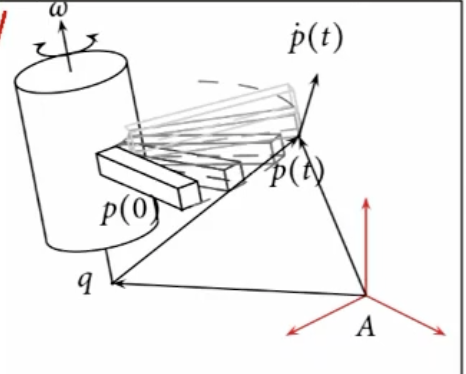
\includegraphics[width=250px]{rotato.png}

It satisfies this differential equation:
\[ \dot{p}(t) = \omega \cross (p(t) - q) = \hat{\omega} p - \omega \cross q \]
Which can be written as:
\[ \begin{bmatrix} \dot{p} \\ 0 \end{bmatrix} = \begin{bmatrix}
    \hat{\omega} & - \omega \cross q \\ 0 & 0
\end{bmatrix} \begin{bmatrix}
    p \\ 1
\end{bmatrix} \]
Which is then:
\[ \dot{\bar{p}} = \hat{\xi} \bar{p}(t) \implies \bar{p}(t) = e^{\hat{\xi} t} \bar{p}(0) \]